
% !TEX root = ./paper.tex


%% \section{Sample \tcpls sessions}

%% \tcpls defines several messages that \tcpls hosts can exchange during a \tcpls session. Each of these messages is placed inside an encrypted and authenticated \tls record with a dedicated True Type. The following \tcpls messages are defined in our prototype:

%% \begin{itemize}

%% \item BPF: this \tcpls message contains eBPF bytecode which can be injected in the TCP stack of the receiving host
%% \item MULTIHOMING\_v6: this \tcpls message contains an IPv6 address
%% \item MULTIHOMING\_v4: this \tcpls message contains an IPv4 address
%% \item SESSID: this message contains a variable length identifier for the current \tcpls session
%% \item COOKIE: this \tcpls message contains a cookie
%% \item MPJOIN: this \tcpls message contains \tcpls session identifier and a cookir
%% \item DATA\_ACK: this \tcpls message contains the sequence number of the last record  received over the session
%% \item FAILOVER: \todo{explain}
%% \item FAILOVER\_END: \todo{explain}
%% \item STREAM\_ATTACH: this \tcpls message attaches the stream identifier provided as parameter to the \tcpls session
%% \item STREAM\_CLOSE: this \tcpls message detaches the stream identifier provided as parameter from the \tcpls session
%% \item STREAM\_CLOSE\_ACK: this \tcpls message confirms that the stream identifier provided as parameter has been detached from the \tcpls session
%% \item USER\_TIMEOUT: this \tcpls message encodes the TCP User Timeout option defined \cite{rfc5482}
%% \item TRANSPORT\_NEW: \todo{explain}
%% \item TRANSPORT\_UPDATE: \todo{explain}

%% \end{itemize}

%% We now provide some sample \tcpls sessions to illustrate the operation of the protocol.


\section{The \tcpls API}
\label{appendix:api}

To illustrate \tcpls API's flexibility, we consider a simple
use case inspired by Happy Eyeballs~\cite{rfc8305}. This technique is
used by web browsers when interacting with dual-stack servers. They
try to establish \tcp connections using IPv4 and IPv6 and prefer the
one that offers the lowest latency. This avoids problems when an address
family is broken on a path but not the other and sometimes results in
lower latency~\cite{bajpai2019longitudinal}.

\begin{figure}[!t]
  \resizebox{0.49\textwidth}{!}{%
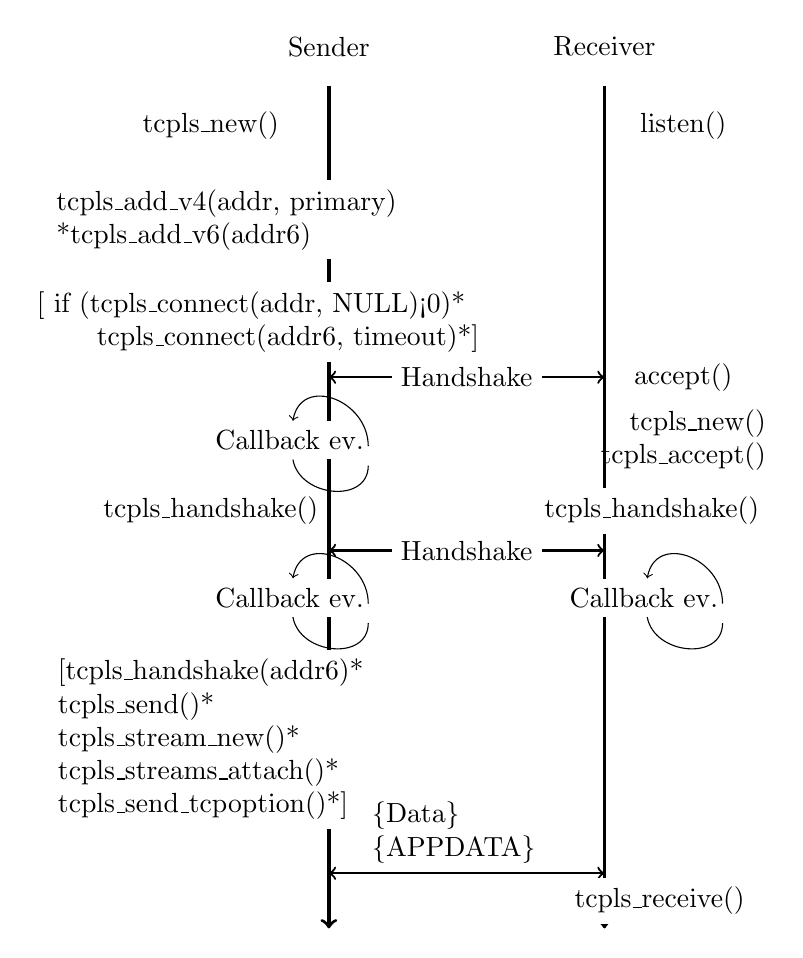
\begin{tikzpicture}
   \colorlet{lightgray}{black!20}
   \tikzstyle{arrow} = [thick,->,>=stealth]
   \tikzset{state/.style={rectangle, dashed, draw, fill=white} }
   \node[black, fill=white] at (0.5,10) {Sender};
   \node[black, fill=white] at (4,10) {Receiver};
   \draw[very thick,->] (0.5,9.5) -- (0.5,-1.2);
   \draw[very thick,->] (4,9.5) -- (4,-1.2);
   \node at (-1,9) {tcpls\_new()};
   \node at (5, 9) {listen()};
   \node[align=left, fill=white] at (-0.8,7.8) {tcpls\_add\_v4(addr,
     primary)\\*tcpls\_add\_v6(addr6)};
   \node[fill=white, align=left] at (-0.4,6.5) {[ if (tcpls\_connect(addr,
     NULL)<0)*\\
     \indent~~tcpls\_connect(addr6, timeout)*]};
   \draw[black, thick, <->] (0.5,5.8) -- (4,5.8) node [midway, fill=white] {\tcp Handshake};
   \node[fill=white] at (0,5) (Callback) {Callback ev.};
   \node at (1,4.8) (here) {};
   \draw [->] (Callback) to[out=-80, in=-90,looseness=1.3] (here)
   to[out=90,in=80,looseness=1.5] (Callback);
   \node at (5, 5.8) {accept()};
   \node[align=right] at (5, 5) {tcpls\_new()\\tcpls\_accept()};
   \node at (-1,4.1) {tcpls\_handshake()};
   \node[fill=white] at (4.6,4.1) {tcpls\_handshake()};
   \draw[black, thick, <->] (0.5,3.6) -- (4,3.6) node [midway, fill=white] {\tcpls Handshake};
   \node[fill=white] at (0,3) (CB2) {Callback ev.};
   \node at (1,2.8) (here2) {};
   \draw [->] (CB2) to[out=-80, in=-90,looseness=1.3] (here2)
   to[out=90,in=80,looseness=1.5] (CB2);
   \node[fill=white] at (4.5,3) (CB3) {Callback ev.};
   \node at (5.5,2.8) (here3) {};
   \draw [->] (CB3) to[out=-80, in=-90,looseness=1.3] (here3)
   to[out=90,in=80,looseness=1.5] (CB3);
   \node[fill=white, align=left] at (-1, 1.2)
   {[tcpls\_handshake(addr6)*\\tcpls\_send()*\\tcpls\_stream\_new()*\\tcpls\_streams\_attach()*\\tcpls\_send\_tcpoption()*]};
   \draw[black, thick, <->] (0.5,-0.5) -- (4,-0.5) node [midway, fill=white,
   above, text width=2.4cm]
   {\{\tcpls Data\} \{APPDATA\}};
   \node[fill=white] at (4.7,-0.85) {tcpls\_receive()};
\end{tikzpicture}
}
\caption{API Workflow example. * means optional call, [ ] means optional call flow, and \{ \} means encrypted.}
  \label{fig:api}
\end{figure}

Fig.~\ref{fig:api} shows an example of our current API workflow. The API can
handle explicit multipath techniques such as Happy Eyeball by chaining
\texttt{tcpls\_connect()} with an appropriate timeout of 50ms, as shown in the
Figure. \tcpls lets the application explicitly choose the multipath mesh by
calling several times \texttt{tcpls\_connect(src, dest,timeout)};. The
application may configure callbacks to connection events that would occur within
\tcpls, such as a connection establishment, a stream attachment, a multipath
join, the reception of a \tcp option to tune \tcp, and more. When multiple
streams are attached to multiple \tcp connections, the application may configure
various \tcpls behaviours. Among them, we support HOL-blocking avoidance,
aggregation of bandwidth with multipathing, connection failover, and connection
migration. Note that, HOL-blocking avoidance is incompatible with the
aggregation of bandwidth with multipathing (the application can do either one
but not both at the same time).

\section{Capability Comparison}


Table~\ref{table:tcplsvsquic} compares the features supported by
\tcp, \mptcp, \tls/\tcp, \quic and \tcpls. \quic and \tcpls are very similar in their
capabilities. They mainly differ in their semantic. \tcpls's semantic is to let
the applications make the decision, and we design its API to fulfill this goal.
That is, the meaning of \tcpls is to offer advanced, extensible and secure
transport-layer functionalities on top of \tcp, while exposing a simple but
powerful API to let the application composes the properties its transport should
have.

Note that several of the features suggested by \tcpls are also suggested on \tcp
or \quic via research works such as a new socket API for explicit \mptcp
\cite{hesmans2016enhanced}, or eBPF plugins in
\quic~\cite{de2019pluginizing}.

\begin{table*}[!t]
  \small
  \begin{tabular}{lccccc}
    \toprule
    & \tcp & \mptcp & \tls/\tcp & \quic & \tcpls \\
    \midrule
    Transport reliability & \checkmark & \checkmark & \checkmark & \checkmark & \checkmark \\
    Message conf. and auth.&  \xmark & \xmark & \checkmark & \checkmark & \checkmark \\
    Connection reliability (failover) &  \xmark & \checkmark &\xmark & (\checkmark) & \checkmark \\
    0-RTT & \checkmark & \xmark & (\xmark) & \checkmark  & \checkmark \\
    Session Resumption & \xmark & \xmark & \checkmark & \checkmark & \checkmark \\
    Connection Migration & \xmark & \xmark &\xmark & \checkmark & \checkmark \\
    \multicolumn{5}{l}{Application-exposed features} \\
    \hspace{2em} Streams & \xmark &  \xmark & \xmark & \checkmark & \checkmark \\
    \hspace{2em} Happy eyeballs & \xmark & \xmark & \xmark & \xmark & \checkmark \\
    \hspace{2em} Explicit Multipath & \xmark & \xmark & \xmark & \xmark & \checkmark \\
    \hspace{2em} App-level Con. migration & \xmark & \xmark & \xmark & \xmark & \checkmark \\
    \hspace{2em} kernel eBPF Pluginization & \xmark & \xmark & \xmark & \xmark & \checkmark \\
    Resilience to HOL blocking & \xmark & \xmark & \xmark & \checkmark  & \checkmark \\
    Secure Connection Closing & \xmark &  \xmark & \xmark & \checkmark & \checkmark \\
    \bottomrule
  \end{tabular}
  \caption{Protocol features comparison. (\xmark) means that the feature is
    available, but not straightforward to use. (\checkmark) means that the
  feature is partially available and under development.}
  \label{table:tcplsvsquic}
\end{table*}

\section{Failover Protocol}

Figure~\ref{fig:protocol_example} gives a selected set of messages during the
establishment of a \tcpls session, a file transfer and a network failure with
the failover feature enabled by default on both peer. First, during the \tcpls
handshake, we may observe the \tls encrypted extensions \texttt{Cookies}, \texttt{Sessid},
\texttt{Multihoming v6} and \texttt{User Timeout} sent with the
\texttt{ServerHello} messages. The multihoming v6 extension announces an
alternative address to the client, and the User Timeout \tcpls extension
announces to the peer that it should not wait more than the $X$ ms to expect
more data to read. In this experiment, the User Timeout is $250ms$, and
should in practice be an upper bound of the server-to-client path latency.
After the handshake is finished, the Server proceeds to attach a stream and
begins to send the file content within TLS APPDATA records. The clients sends
special \tcpls DATA\_ACK to acknowledge the received records. In this
experiment, the network suffers a failure after around $16s$ of transfer. The client performs a
Join \tcpls handshake over the v6 address received during the \tcpls initial
handshake and play the Failover protocol over the new path. Both peer
resynchronize their decrypting sequence number and replay the records that have
been lost on the first network path's failure. When they sent all lost records,
a FAILOVER\_END message is sent and the stream is recovered. The Server can
proceed to send the data and finishes by securly closing the stream.

To be extra clear on any security concern, different records are never encrypted
with the same sequence number, nor any record is encrypted twice or decrypted
twice.

% Agents
\def\Client{Client}
\def\Server{Server}
\def\Inactivity{Inactivity}
\def\Event{Event}


\begin{figure*}[!t]
 \begin{center}
   \begin{tiny}
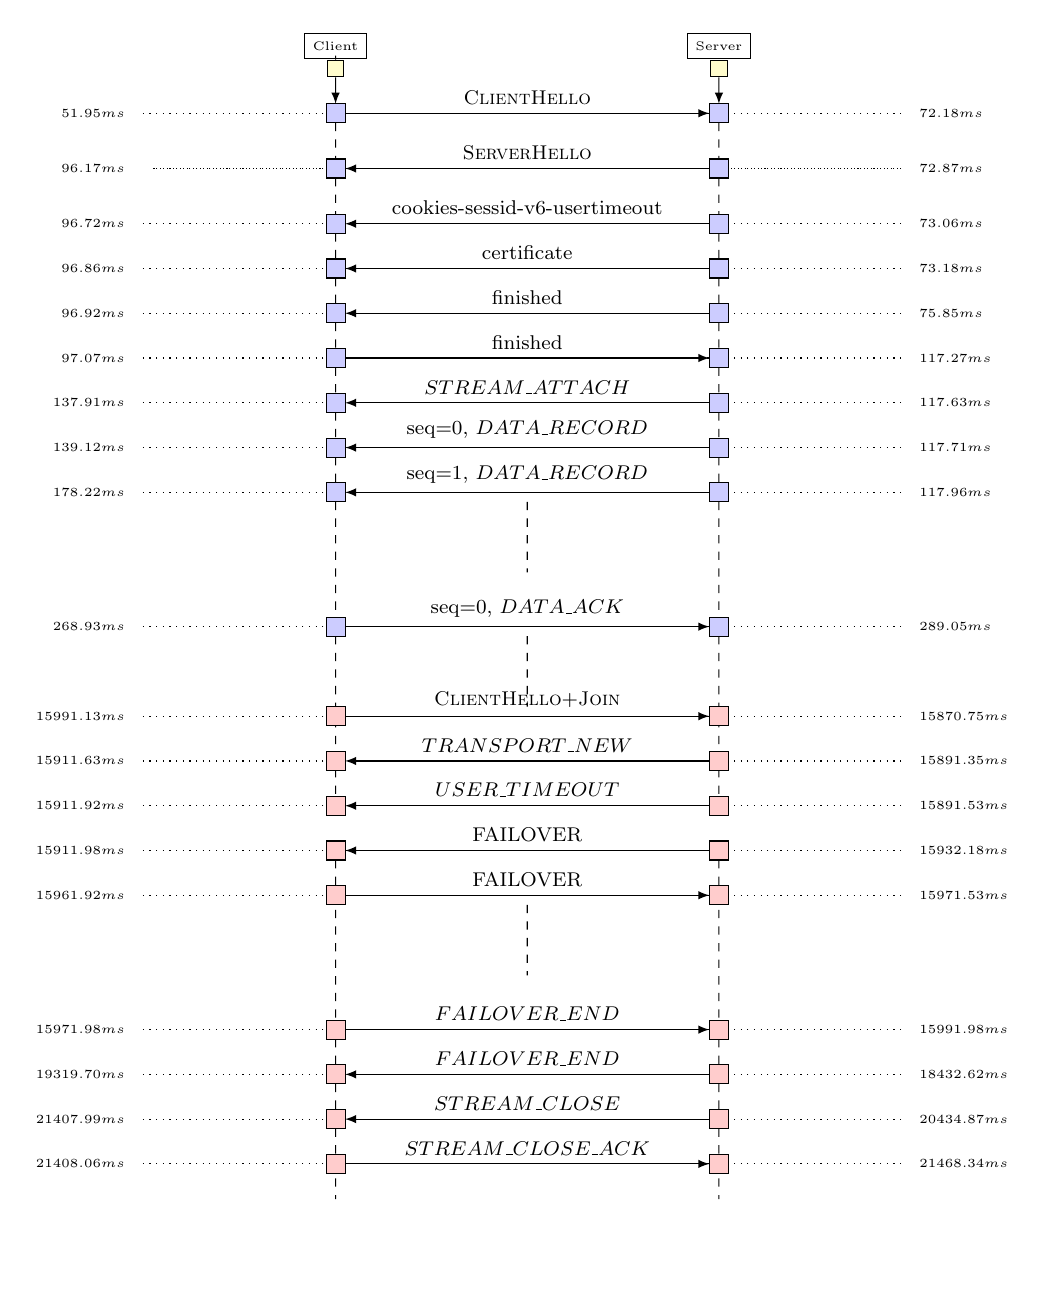
\begin{tikzpicture}[every node/.style={font=\tiny, minimum height=0.03cm,minimum width=0.03cm},scale=0.90, transform shape]
\tikzset{label/.style={align=center,minimum height=0.5cm,minimum width=5mm}}
\node [matrix, very thin,column sep=2.2cm,row sep=0.05cm] (matrix) at (0,0) {
  & \node(0,0) (\Client) {}; & \node(0,0) (\Inactivity) {};  & \node(0,0) (\Server) {};  & \\
  & \node(0,0) (\Client 0) {}; & & \node(0,0) (\Server 0) {};  & \\
  \node(0,0) (u1 left) {}; & & & &   \node(0,0) (u1 right) {};\\
  \node(0,0) (t0 left) {}; & \node(0,0) (\Client 1) {}; & \node(0,0) (\Event 1) {}; & \node(0,0) (\Server 1) {};  & \node(0,0) (t0 right) {};\\
   \node(0,0) (u1 left) {}; & & & &   \node(0,0) (u1 right) {};\\
 \node[label] (t1 left) {}; & \node(0,0) (\Client 2) {}; & \node(0,0) (\Event 2) {}; & \node(0,0) (\Server 2) {};  &\node(0,0) (t1 right) {}; \\
  \node(0,0) (u2 left) {}; & & & &   \node(0,0) (u2 right) {};\\
\node(0,0) (t2 left) {};  & \node(0,0) (\Client 3) {}; & \node(0,0) (\Event 3) {}; & \node(0,0) (\Server 3) {};  & \node(0,0) (t2 right) {};\\
  \node(0,0) (u3 left) {}; & & & &   \node(0,0) (u3 right) {};\\
  \node(0,0) (t3 left) {}; & \node(0,0) (\Client 4) {}; & \node(0,0) (\Event 4) {}; & \node(0,0) (\Server 4) {};  &  \node(0,0) (t3 right) {};\\
  \node(0,0) (u4 left) {}; & & & &   \node(0,0) (u4 right) {};\\
 \node(0,0) (t4 left) {}; & \node(0,0) (\Client 5) {}; & \node(0,0) (\Event 5) {}; & \node(0,0) (\Server 5) {};  & \node(0,0) (t4 right) {}; \\
  \node(0,0) (u5 left) {}; & & & &   \node(0,0) (u5 right) {};\\
 \node(0,0) (t5 left) {}; & \node(0,0) (\Client 6) {}; & \node(0,0) (\Event 6) {}; & \node(0,0) (\Server 6) {};  & \node(0,0) (t5 right) {};\\
  \node(0,0) (u6 left) {}; & & & &   \node(0,0) (u6 right) {};\\
 \node(0,0) (t6 left) {};  & \node(0,0) (\Client 7) {}; & \node(0,0) (\Event 7) {}; & \node(0,0) (\Server 7) {};  & \node(0,0) (t6 right) {};\\
  \node(0,0) (u7 left) {}; & & & &   \node(0,0) (u7 right) {};\\
 \node(0,0) (t7 left) {}; & \node(0,0) (\Client 8) {}; & \node(0,0) (\Event 8) {}; & \node(0,0) (\Server 8) {};  &  \node(0,0) (t7 right) {}; \\
  \node(0,0) (u8 left) {}; & & & &   \node(0,0) (u8 right) {};\\
  \node(0,0) (t8 left) {}; & \node(0,0) (\Client 9) {}; & \node(0,0) (\Event 9) {}; & \node(0,0) (\Server 9) {};  & \node(0,0) (t8 right) {};\\
  \node(0,0) (u9 left) {}; & & & &   \node(0,0) (u9 right) {};\\
 \node(0,0) (t9 left) {}; & \node(0,0) (\Client 10) {}; & \node(0,0) (\Event 10) {}; & \node(0,0) (\Server 10) {};  & \node(0,0) (t9 right) {};\\
  \node(0,0) (u10 left) {}; & & & &   \node(0,0) (u10 right) {};\\
  \node(0,0) (t10 left) {}; & \node(0,0) (\Client 11) {}; & \node(0,0) (\Event 11) {}; & \node(0,0) (\Server 11) {};  & \node(0,0) (t10 right) {};\\
  \node(0,0) (u11 left) {}; & & & &   \node(0,0) (u11 right) {};\\
  \node(0,0) (t11 left) {}; & \node(0,0) (\Client 12) {}; & \node(0,0) (\Event 12) {}; & \node(0,0) (\Server 12) {};  & \node(0,0) (t11 right) {};\\
   \node(0,0) (t12 left) {}; & & & &   \node(0,0) (t12 right) {};\\
  & \node(0,0) (\Client 13) {}; & \node(0,0) (\Event 13) {}; & \node(0,0) (\Server 13) {};  & \\
   \node(0,0) (u13 left) {}; & & & &   \node(0,0) (u13 right) {};\\
 \node(0,0) (t13 left) {}; & \node(0,0) (\Client 14) {}; & \node(0,0) (\Event 14) {}; & \node(0,0) (\Server 14) {};  &  \node(0,0) (t13 right) {};\\
   \node(0,0) (u14 left) {}; & & & &   \node(0,0) (u14 right) {};\\
 \node(0,0) (t14 left) {}; & \node(0,0) (\Client 15) {}; & \node(0,0) (\Event 15) {}; & \node(0,0) (\Server 15) {};  & \node(0,0) (t14 right) {};\\
   \node(0,0) (u15 left) {}; & & & &   \node(0,0) (u15 right) {};\\
  \node(0,0) (t15 left) {};  & \node(0,0) (\Client 16) {}; & \node(0,0) (\Event 16) {}; & \node(0,0) (\Server 16) {};  & \node(0,0) (t15 right) {};\\
   \node(0,0) (u16 left) {}; & & & &   \node(0,0) (u16 right) {};\\
 \node(0,0) (t16 left) {}; & \node(0,0) (\Client 17) {}; & \node(0,0) (\Event 17) {}; & \node(0,0) (\Server 17) {};  & \node(0,0) (t16 right) {};\\
  \node(0,0) (u17 left) {}; & & & &   \node(0,0) (u17 right) {};\\
 \node(0,0) (t17 left) {};  & \node(0,0) (\Client 18) {}; & \node(0,0) (\Event 18) {}; & \node(0,0) (\Server 18) {};  &\node(0,0) (t17 right) {}; \\
  \node(0,0) (t18 left) {}; & & & &   \node(0,0) (t18 right) {};\\
  & \node(0,0) (\Client 19) {}; & \node(0,0) (\Event 19) {}; & \node(0,0) (\Server 19) {};  & \\
  \node(0,0) (t20 left) {}; & & & &   \node(0,0) (t20 right) {};\\
  & \node(0,0) (\Client 20) {}; & \node(0,0) (\Event 20) {}; & \node(0,0) (\Server 20) {};  & \\
  \node(0,0) (u21 left) {}; & & & &   \node(0,0) (u21 right) {};\\
  \node(0,0) (t21 left) {};& \node(0,0) (\Client 21) {}; & \node(0,0) (\Event 21) {}; & \node(0,0) (\Server 21) {};  & \node(0,0) (t21 right) {};\\
  \node(0,0) (u22 left) {}; & & & &   \node(0,0) (u22 right) {};\\
 \node(0,0) (t22 left) {}; & \node(0,0) (\Client 22) {}; & \node(0,0) (\Event 22) {}; & \node(0,0) (\Server 22) {};  &  \node(0,0) (t22 right) {};\\
  \node(0,0) (u23 left) {}; & & & &   \node(0,0) (u23 right) {};\\
 \node(0,0) (t23 left) {}; & \node(0,0) (\Client 23) {}; & \node(0,0) (\Event 23) {}; & \node(0,0) (\Server 23) {};  & \node(0,0) (t23 right) {};\\
  \node(0,0) (u24 left) {}; & & & &   \node(0,0) (u24 right) {};\\
 \node(0,0) (t24 left) {}; & \node(0,0) (\Client 24) {}; & \node(0,0) (\Event 24) {}; & \node(0,0) (\Server 24) {};  & \node(0,0) (t24 right) {};\\
  \node(0,0) (t25 left) {}; & & & &   \node(0,0) (t25 right) {};\\
  & \node(0,0) (\Client 25) {}; & \node(0,0) (\Event 25) {}; & \node(0,0) (\Server 25) {};  & \\
  \node(0,0) (t26 left) {}; & & & &   \node(0,0) (t26 right) {};\\
  & \node(0,0) (\Client 26) {}; & \node(0,0) (\Event 26) {}; & \node(0,0) (\Server 26) {};  & \\
};

% Agents labels
\fill
	(\Client) node[draw,fill=white] {\Client}
	(\Server) node[draw,fill=white] {\Server};

% Horizontal time lines
\draw [dotted]
  (t0 left) -- (t0 right) node[right] {$72.18ms$}
  (t0 right) -- (t0 left) node[left] {$51.95ms$}
  (t1 left) -- (t1 right) node[right] {$72.87ms$}
  (t1 right) -- (t1 left) node[left] {$96.17ms$}
  (t2 left) -- (t2 right) node[right] {$73.06ms$}
  (t2 right) -- (t2 left) node[left] {$96.72ms$}
  (t3 left) -- (t3 right) node[right] {$73.18ms$}
  (t3 right) -- (t3 left) node[left] {$96.86ms$}
  (t4 left) -- (t4 right) node[right] {$75.85ms$}
  (t4 right) -- (t4 left) node[left] {$96.92ms$}
  (t5 left) -- (t5 right) node[right] {$117.27ms$}
  (t5 right) -- (t5 left) node[left] {$97.07ms$}
  (t6 left) -- (t6 right) node[right] {$117.63ms$}
  (t6 right) -- (t6 left) node[left] {$137.91ms$}
  (t7 left) -- (t7 right) node[right] {$117.71ms$}
  (t7 right) -- (t7 left) node[left] {$139.12ms$}
  (t8 left) -- (t8 right) node[right] {$117.96ms$}
  (t8 right) -- (t8 left) node[left] {$178.22ms$}
  (t11 left) -- (t11 right) node[right] {$289.05ms$}
  (t11 right) -- (t11 left) node[left] {$268.93ms$}
  (t13 left) -- (t13 right) node[right] {$15870.75ms$}
  (t13 right) -- (t13 left) node[left] {$15991.13ms$}
  (t14 left) -- (t14 right) node[right] {$15891.35ms$}
  (t14 right) -- (t14 left) node[left] {$15911.63ms$}
  (t15 left) -- (t15 right) node[right] {$15891.53ms$}
  (t15 right) -- (t15 left) node[left] {$15911.92ms$}
  (t16 left) -- (t16 right) node[right] {$15932.18ms$}
  (t16 right) -- (t16 left) node[left] {$15911.98ms$}
  (t17 left) -- (t17 right) node[right] {$15971.53ms$}
  (t17 right) -- (t17 left) node[left] {$15961.92ms$}
  (t21 left) -- (t21 right) node[right] {$15991.98ms$}
  (t21 right) -- (t21 left) node[left] {$15971.98ms$}
  (t22 left) -- (t22 right) node[right] {$18432.62ms$}
  (t22 right) -- (t22 left) node[left] {$19319.70ms$}
  (t23 left) -- (t23 right) node[right] {$20434.87ms$}
  (t23 right) -- (t23 left) node[left] {$21407.99ms$}
  (t24 left) -- (t24 right) node[right] {$21468.34ms$}
  (t24 right) -- (t24 left) node[left] {$21408.06ms$};

\draw
  (\Client 0)
    node[draw,rectangle,fill=yellow!20, rotate=-90]
      (\Client Timeline In) {}
    node[below right] {}
  (\Server 0)
    node[draw,rectangle,fill=yellow!20, rotate=-90]
      (\Server Timeline In) {}
    node[below right] {};

% Vertical flows
\draw [-latex] (\Client Timeline In.east) -- (\Client 1);
\draw [-latex] (\Server Timeline In.east) -- (\Server 1);

\draw [dashed]
  (\Client) -- (\Client Timeline In.west)
  (\Client 1) -- (\Client 2)
  (\Server 1) -- (\Server 2)
  (\Server 2) -- (\Server 3)
  (\Client 2) -- (\Client 3)
  (\Server 3) -- (\Server 4)
  (\Client 3) -- (\Client 4)
  (\Server 4) -- (\Server 5)
  (\Client 4) -- (\Client 5)
  (\Server 5) -- (\Server 6)
  (\Client 5) -- (\Client 6)
  (\Server 6) -- (\Server 7)
  (\Client 6) -- (\Client 7)
  (\Server 7) -- (\Server 8)
  (\Client 7) -- (\Client 8)
  (\Server 8) -- (\Server 9)
  (\Client 8) -- (\Client 9)
  (\Server 9) -- (\Server 12)
  (\Client 9) -- (\Client 12)
  (\Server 12) -- (\Server 13)
  (\Client 12) -- (\Client 13)
  (\Server 12) -- (\Server 16)
  (\Client 12) -- (\Client 16)
  (\Server 17) -- (\Server 21)
  (\Client 17) -- (\Client 21)
  (\Server 21) -- (\Server 22)
  (\Client 21) -- (\Client 22)
  (\Server 22) -- (\Server 23)
  (\Client 22) -- (\Client 23)
  (\Server 23) -- (\Server 25)
  (\Client 23) -- (\Client 25)

  (\Event 9) -- (\Event 11)
  (\Event 12) -- (\Event 14)
  (\Event 18) -- (\Event 20);

% Blocks (Budget constraints)
\filldraw[fill=blue!20]
  (\Server 1.north west) rectangle (\Server 1.south east)
  (\Client 1.north west) rectangle (\Client 1.south east)
  (\Server 2.north west) rectangle (\Server 2.south east)
  (\Client 2.north west) rectangle (\Client 2.south east)
  (\Server 3.north west) rectangle (\Server 3.south east)
  (\Client 3.north west) rectangle (\Client 3.south east)
  (\Server 4.north west) rectangle (\Server 4.south east)
  (\Client 4.north west) rectangle (\Client 4.south east)
  (\Server 5.north west) rectangle (\Server 5.south east)
  (\Client 5.north west) rectangle (\Client 5.south east)
  (\Server 6.north west) rectangle (\Server 6.south east)
  (\Client 6.north west) rectangle (\Client 6.south east)
  (\Server 7.north west) rectangle (\Server 7.south east)
  (\Client 7.north west) rectangle (\Client 7.south east)
  (\Server 8.north west) rectangle (\Server 8.south east)
  (\Client 8.north west) rectangle (\Client 8.south east)
  (\Server 9.north west) rectangle (\Server 9.south east)
  (\Client 9.north west) rectangle (\Client 9.south east)
  (\Server 12.north west) rectangle (\Server 12.south east)
  (\Client 12.north west) rectangle (\Client 12.south east);


\filldraw[fill=red!20]
  (\Server 14.north west) rectangle (\Server 14.south east)
  (\Client 14.north west) rectangle (\Client 14.south east)
  (\Server 15.north west) rectangle (\Server 15.south east)
  (\Client 15.north west) rectangle (\Client 15.south east)
  (\Server 16.north west) rectangle (\Server 16.south east)
  (\Client 16.north west) rectangle (\Client 16.south east)
  (\Server 17.north west) rectangle (\Server 17.south east)
  (\Client 17.north west) rectangle (\Client 17.south east)
  (\Server 18.north west) rectangle (\Server 18.south east)
  (\Client 18.north west) rectangle (\Client 18.south east)
  (\Server 21.north west) rectangle (\Server 21.south east)
  (\Client 21.north west) rectangle (\Client 21.south east)
  (\Server 22.north west) rectangle (\Server 22.south east)
  (\Client 22.north west) rectangle (\Client 22.south east)
  (\Server 23.north west) rectangle (\Server 23.south east)
  (\Client 23.north west) rectangle (\Client 23.south east)
  (\Server 24.north west) rectangle (\Server 24.south east)
  (\Client 24.north west) rectangle (\Client 24.south east);

\draw [-latex] (\Client 1) -- (\Server 1);
\draw [-latex] (\Server 2) -- (\Client 2);
\draw [-latex] (\Server 3) -- (\Client 3);
\draw [-latex] (\Server 4) -- (\Client 4);
\draw [-latex] (\Server 5) -- (\Client 5);
\draw [-latex] (\Client 6) -- (\Server 6);
\draw [-latex] (\Server 7) -- (\Client 7);
\draw [-latex] (\Server 8) -- (\Client 8);
\draw [-latex] (\Server 9) -- (\Client 9);
\draw [-latex] (\Client 12) -- (\Server 12);
\draw [-latex] (\Client 14) -- (\Server 14);
\draw [-latex] (\Server 15) -- (\Client 15);
\draw [-latex] (\Server 16) -- (\Client 16);
\draw [-latex] (\Server 17) -- (\Client 17);
\draw [-latex] (\Client 18) -- (\Server 18);
\draw [-latex] (\Client 21) -- (\Server 21);
\draw [-latex] (\Server 22) -- (\Client 22);
\draw [-latex] (\Server 23) -- (\Client 23);
\draw [-latex] (\Client 24) -- (\Server 24);



% Flows Labels
\fill
  (\Event 1)
    node[above,font=\footnotesize] {\textsc{ClientHello}}
    node[font=\footnotesize, below] {}
    (\Event 2)
    node[above,font=\footnotesize] {\textsc{ServerHello}}
    node[font=\footnotesize, below] {}
    (\Event 3)
    node[above,font=\footnotesize] {cookies-sessid-v6-usertimeout}
    node[font=\footnotesize, below] {}
    (\Event 4)
    node[above,font=\footnotesize] {certificate}
    node[font=\footnotesize, below] {}
    (\Event 5)
    node[above,font=\footnotesize] {finished}
    node[font=\footnotesize, below] {}
    (\Event 6)
    node[above,font=\footnotesize] {finished}
    node[font=\footnotesize, below] {}
    (\Event 7)
    node[above,font=\footnotesize] {$STREAM\_ATTACH$}
    node[font=\footnotesize, below] {}
     (\Event 8)
    node[above,font=\footnotesize] {seq=0, $DATA\_RECORD$}
    node[font=\footnotesize, below] {}
    (\Event 9)
    node[above,font=\footnotesize] {seq=1, $DATA\_RECORD$}
    node[font=\footnotesize, below] {}
     (\Event 12)
    node[above,font=\footnotesize] {seq=0, $DATA\_ACK$}
    node[font=\footnotesize, below] {}
    (\Event 14)
    node[above,font=\footnotesize] {\textsc{ClientHello}+\textsc{Join}}
    node[font=\footnotesize, below] {}
    (\Event 15)
    node[above,font=\footnotesize] {$TRANSPORT\_NEW$}
    node[font=\footnotesize, below] {}
    (\Event 16)
    node[above,font=\footnotesize] {$USER\_TIMEOUT$}
    node[font=\footnotesize, below] {}
    (\Event 17)
    node[above,font=\footnotesize] {FAILOVER}
    node[font=\footnotesize, below] {}
    (\Event 18)
    node[above,font=\footnotesize] {FAILOVER}
    node[font=\footnotesize, below] {}
    (\Event 21)
    node[above,font=\footnotesize] {$FAILOVER\_END$}
    node[font=\footnotesize, below] {}
    (\Event 22)
    node[above,font=\footnotesize] {$FAILOVER\_END$}
    node[font=\footnotesize, below] {}
    (\Event 23)
    node[above,font=\footnotesize] {$STREAM\_CLOSE$}
    node[font=\footnotesize, below] {}
    (\Event 24)
    node[above,font=\footnotesize] {$STREAM\_CLOSE\_ACK$}
    node[font=\footnotesize, below] {};

\end{tikzpicture}
\end{tiny}
\end{center}
  \caption{Example of record messages exchanged covering the attachment of a
    new stream, the reception of DATA\_RECORD containing application payload, the exchange of DATA\_ACK, a Failover
    event in which the stream is recovered and finally a secure closing the
    connection. Real trace captured with qlog and pruned to only show
    interesting messages}
  \label{fig:protocol_example}
\end{figure*}

\section{Multipath Aggregation}
\label{appendix:aggr}

Figure~\ref{fig:aggregation_1500bytes_records} shows the same experiment than
the one provided in our evaluation Section~\ref{sec:bwaggr}. However, we use
1500 bytes record size for \tcpls in order to demonstrate that the
irregularities are mainly due to the payload chunk size that the reordering
algorithm has to manipulate. The larger the records are, the bigger
the payload chunk size is, and higher irregularities should be observed. We
observe here a steady goodput with several large irregularities, which is a
progress compared to Figure~\ref{fig:multipath_aggregation}. However, large
peaks remain, which are probably linked to the state of advancement of our
research prototype: several bugs might remain.

\begin{figure}
  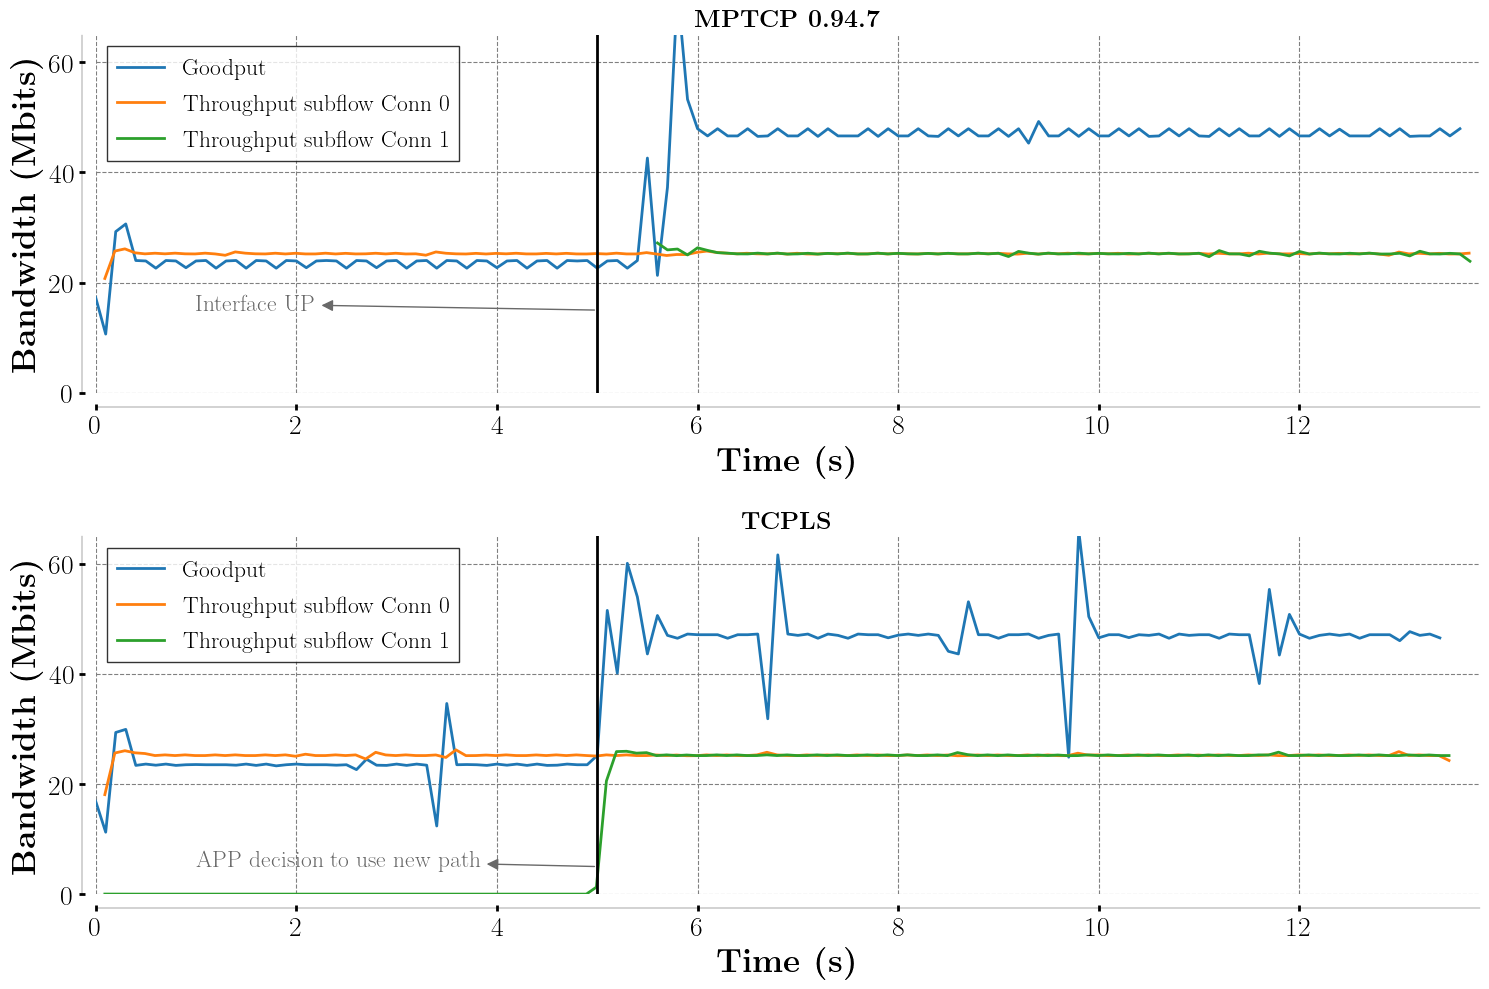
\includegraphics[width=\columnwidth]{figures/aggregate_1500bytes_records_dual.png}
  \caption{\tcpls path aggregation with $1500$ bytes record size, compared to
    \tls over \mptcp with 16384 bytes record size}
  \label{fig:aggregation_1500bytes_records}
\end{figure}
